% !TeX spellcheck = sk_SK
 


\section{Analýza problému} 

  

\subsection{Petriho siete} % not called Petriflow 

 Carl Adam Petri založil koncept Petriho sietí v roku 1962 vo svojej dizertačnej práci - Komunikácia s Automatmi - na Technickej Univerzite v Darmstadte. Ďalším výskumom sa z pôvodného konceptu ktorý bol určený na modelovanie analýzu komunikačných systémov vyvynul nástroj, ktorý sa používa naprieč monými oblastiami najmä na modelovanie papalelných a distribuovaných systémov. 
 
 Základné Petriho siete pozostávajú z prechodov, miest a hrán. 
 %TODO rozumna definica PN
  
\subsection{Petriflow} % not called Petriflow 
\cite{petriflow_clanok}
Formalizmus Petriflow je rozšírenie Petriho sietí, ktoré bolo navrhnuté na modelovanie komplexných biznisových procesov. Je vvyíjaný spoločnosťou Netgrif na základe dlhodobých skúseností s klientami, ktorý pomocou tohto formalizmu modelujú svoje biznis procesy, ktoré sú následne zavedené do používania. 
%TODO bleh
%TODO komu dat credit?
%TODO cite diplomka
Formalizmus Petriflow rozširuje Petriho siete o daľsie kompnenty. Ako základ berie Petriho siete obohatené reset, inihibitor a read hrany. Aby sa dali modelovať moderné biznis procesy pridáva Petriflow do tohto modelu roly, dátové polia a akcie. 
Roly definujú kto je oprávnený spúšťať rôzne prechody. 
Dátové polia definujú štruktúru dát ktoré každá inštanica procesu obsahuje počas svojho behu.
Akcie definujú vsťahy a interakcie medzi jednotlivými dátovými poliami a prechodmi.

V klacických petriho sieťach je spustenie prechodu vždy atomická operáci. Petriflow obsahuje 2 typy prechodov udalostné precohdy, ktoré sú rovnako  ako v klasických PN sieťach atomické, avšak vždy ich spúšťa nejaká osoba(používaťeľ) v systéme. Druhý typ prechodu je úloha. Úlohu môžeme vnímať ako podsieť na obrázku \ref{task}. Na začiatku je úloha nepridelená, ako prvý krok je potrebné ju niekomu (aj sebe) prideliť. Následne môže toto pridelenie zrušiť, prideliť inej osobe, alebo úlohu dokončiť
%todo - permission to assign/cancel/delegate/finish


\begin{figure}[!htbp]
 	\centering
 	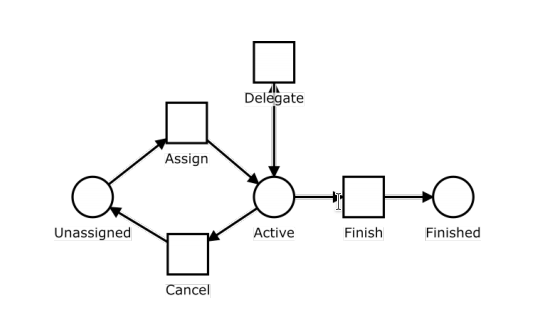
\includegraphics[width=6cm]{img/task_transition.png}
 	\caption{Úloha}
 	\label{task}
\end{figure} 


  

\subsection{Aplikačné rozhranie} 

Majme procesne orientovaný ststém ktorý implementuje procesy, popísane v Petriflow. S takýmto systémom používateľia interagujú iba presne popísaným spôsobom a to spúšťaním prechodov ktoré majú podľa svojich rolí oprávnenie spúšťať (delegovať, dokončiť,... ). Pri dokončení úlohy (prechodu) musí používateľ poskytnúť dáta popísané v dátových poliach. 
Keďže formalizmus Petriflow je schopný takýmto spôsobom popísať všetky interakcie používateľa so systémom je možné na jeho základe vygenerovať aj aplikačné rozhranie. Toto rozhranie sprístupní systém mimo jeho domény, zaručí autorizáciu podľa rolí, poskytne dokumentáciu o svojej štruktúre(a tým pádom aj štruktúre procesu) a zabezpečí validáciu dát, ktoré do systému používateľ odošle.

Ak by rozhranie držalo infromáciu o značkovaní, a teda spustiteľnosti prechodov, mohol by nasať stav kedy aplikačné rozhranie je v stave, ktorý naznačuje, že prechod sa nedá spustiť no procesný server už je v stave, kedy je prechod spustiteľný. Kvôli udržaniu konzistencie dát a predideniu race conditions nemôže aplikačné rozhranie držať informáciu o značkovaní a teda ani spustiteľnosti prechodu.

Aktuálna verzia Petriflow poskytuje relatívne granulárne informácie o autorizácií na vykonávanie akcií pomocou rolí, neobsahuje však introfmáciu o používateľoch ani o tom ktorý používateľ má pridelené aké roly. Na implemetnáciu funkčného aplikačného rozhrania teda bude nutné dorobiť systém ktorý túto informáciu bude obsahovať. 

  
\section{Špecifikácia} 
V tejto kapitole najprv stručne opíšeme hlavnú funkcionalitu navrhovanej aplikácie, potom zadefinujeme funkcionálne a nefunkcionálne požiadavky na aplikáciu. 

Softvér, ktorý sme sa rozhodli implementovať bude slúžiť ako rozhranie medzi procesným serverom a internetom. Bude umožňovať klientovi pripojiť sa na procesný server cez internet, autentifiokvať sa, získať informácie o dátach v prechodoch petriho siete a bude umožňovať modifikovať stav siete (procesu) spúšťaním prechodov. 

  
\subsection{Funkcionálne požiadavky} 

\begin{enumerate} 
    \item Rozhranie bude umožňovať administátorovi registrovať používateľov a priraďovať im roly 
    \item Umožní administrátorovi za behu pridať nové koncevé body a meniť, alebo vymazať aktuálne nasadené koncové body 

    \item Umožní prihlásenie používateľa pomocou štandardného autentifikačného protokolu. 

    \item Autentifikovaným používateľom umožní prístup k dátam z tých prechodov ktoré majú právo čítať podľa ich roly. 

    \item Autentifikovaným používateľom umožní spúšťať prechody ktoré majú právo spúšťať podľa ich roly. 

    \item Pri spúšťaní prechodu prebehne validácia vstupných dát. V prípade nevalidných alebo nekompletných dát nepovolí spustenie prechodu. 

    \item Rozhranie poskytne online dokumentáciu prechodov v sieti, táto dokumentácia bude zahŕňať URL prechodu, potrebné dátové polia na spustenie prechodu a roly, ktoré sú oprávnené prechody spúšťať. 

    \item Rozhranie poskytne aplikačné rozhranie viacerým sieťam s rôznou štruktúrou. A viacerím inštanciám týchto sietí. 
\end{enumerate}     

 

\subsection{Nefunkcionálne požiadavky} 

\begin{enumerate} 
    \item Rozhranie bude škálovateľné 
     
    \item Rozhranie bude zabezpečené štandartnými bezpečnosntými prvkami
    
    \item Rozhranie bude bežať na serveri s operačným systémom Ubuntu 18.04.2 LTS Bionic Beaver poskytnutom Fakultou Elektrotechniky a Informatiky na Slovenskej Technickej Univerzite.  
\end{enumerate} 

  

\section{Návrh} 


% TODO - what have we done in this chapter? 

 

\subsection{Prípady použitia}
Zo špecifikácie vyplývajú nasledovné interakcie používateľa s naším systémom.

\subsubsection{Registrácia modelu}
Prvý prípad použitia \ref{usecase1} je registrácia modelu. Aktér ktorý môže registrovať modely je len administrátor. Pri tejto akcií administrátor poskytne nášmu systému informácie o štruktúre procesu vo formáte petriflow, zoznam používateľov im prislúchajúcich rolí v \acrshort{xml} a unikátny identifikátor siete. 

Pokial chce administrátor upraviť nadadený proces spustí proces registrácie nanovo s upravenými údajmi o sieti, používateľoch a rolách.

Administrátor taktiež môže sieť vymazať. \ref{usecase1}
\begin{figure}[!htbp]
	\centering
	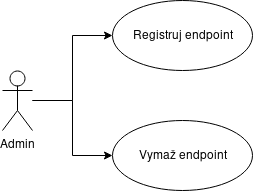
\includegraphics[width=6cm]{img/dp_usecase_1_register.png}
	\caption{Prípad použitia - Registrácia modelu}
	\label{usecase1}
\end{figure} 

\subsubsection{Získanie informácie o prechode}
Keď už sú sieť aj používateľia úspešne zaregistrovaný, si môžu používatelia, vyžiadať \ref{usecase2} informácie o prechode. Tieto informácie budú poskytnuté len používateľovi s rolou oprávnenou na čítanie dát z daného prechodu.

\begin{figure}[!htbp]
	\centering
	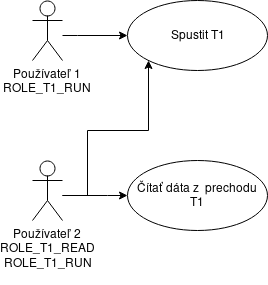
\includegraphics[width=6cm]{img/dp_usecase_2_read_run.png}
	\caption{Prípad použitia - Získanie informácií o prechode}
	\label{usecase2}
\end{figure} 

\subsubsection{Spustenie prechodu}
Používateľia s príslušnými rolami môžu taktie spúšťať \ref{usecase2} prechody. Pri spustení prechodu poskytne používateľ dátové polia potrebné na spustenie prechodu. 

\subsubsection{Autentifikácia}
Z požiadavky na bezpečnosť aplikácie vyplýva ešte prípad použitia, kedy sa používateľ autentifikuje, aby nadobudol identitu rozpoznanú našim systémom a boli mu pridelené roly. 


\subsection{Architektúra} 

Aby sme splnili požiadavku na jednoduché škálovanie aplikácie a pre sprehľadnenie architektúry zvolili sme si architektúru mikroservisov. Táto architektúra pozostáva z viacerých oddelených častí, každá z týchto častí má svoju jasne definovanú funkciu. Takéto mikroservisy sú jednoducho testovateľné, dajú sa nasadzovať postupne a nezávisle od seba a softvér navrhnutý v tejto architektúre býva spravidla robustný a vysoko škálovateľný.  

Softvér sa bude skladať z troch hlavných služieb: generátor, relay bod a autentifikačná služba.
\begin{itemize}
	\item Generator je služba, ktorá bude registrovať a zostavovať koncové body. Je to služba, na ktoú sa pripojí adiministátor, zadá štruktúru siete a zoznam používateľov a rolí. Táto služba následne zaregistuje používateľov a ich roly, vygeneruje kód pre službu relay a túto služnu spustí.
	\item Relay je služba, ktorá obsahuje vygenerovaný kód koncových bodov. Táto služba bude poskytovať dokumentáciu dostupných konových bodov. bude poskytovať samotné koncové body a pri zavolaní koncového bodu sa bude starať o validáciu prijatých dát.
	\item Autentifikačná služba sa stará o autentifikáciu používateľov a pridelovanie rolí použivateľom
	\item Gateway služba poskytuje rozhranie medzi internetom a našou doménou. Vonkajšiemu svetu prezenuje len služby ktoré majú byť dostupné z internetu. Zároveň poskytuje funkcionalitu load balancera. 
\end{itemize}


\begin{figure}[!htbp]
	\centering
	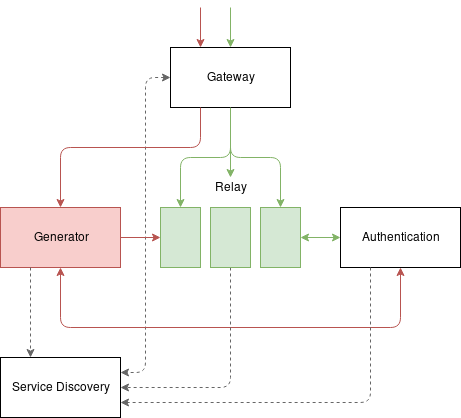
\includegraphics[width=10cm]{img/architecture.png}
	\caption{Architektúra rozhrania}
	\label{architecture}
\end{figure} 


\subsection{Bezpečnosť}
Autentifikáciu v našej aplikácií budeme rieiť pomocou štandartnej knižnice, ktorá poskytuje \acrshort{oauth}. Táto služba bude bežať v samostatnom kontainery a prístup do nej bude len pomocou protokolu oAuth na overovanie klientov a prostredníctvom interného volania na registráciu používateľov.
Ochrana pred neoprávneným prístupom bude dalej relaizovaná pomocou služby gateway. Táto služba bude jediný bod ako sa dá pristúpiť do našej domény z internetu. Služba bude povoľovať len dotazy ktoré špecfikujeme. Ochrana proti neopávnenému prístupu bude taktie realizovaná na vrstve operačného systému pomocou firewallu.
Ochrana proti \acrshort{dos} útokom bude taktiež realizovaná pomocou gateway služby. Táto služba bude slúžiť ako load balancer, a rovnomerne rozdeľovať dotazy medzi inštancie relay servisu tak, aby boli rovnomerne vyťažené. Služba Gateway bude taktie poskytovať ochranu proti priveľkému počtu dotazov od jedného klienta(rate limiting).


\section{Implementácia} 

% TODO 

  

\subsection{Použité technológie} 

  

\subsubsection{Kotlin} 

Kotlin je relatívne nový programovací jazyk, projekt Kotlin bol po prvý krát zverejnený v roku 2011 spoločnosťou JetBrains(Andrey Breslav). Bol vyvinutý ako moderný staticky typovaný jazyk, ktorý podporuje rýchlu kompiláciu do javy. V roku 2017 vyhlásil Google podporu pre Kotlin v operačnom systéme Android.  
Medzi jeho hlavné výhody patrí menší boilerplate (menej zbytočného kódu), a vylepšený systém typovania premenných. V Kotline  môžu byť premenné nulovateľné, to znamená, že kompilátor počita s prípadom, že nulovateľná premenná ešte nieje inizcializovaná. Kompilátor Kotlinu využíva pokročilú logiku na to, aby zistil v ktorých vetvách kódu premenné môžu obsahovať null a v ktorých nie. V prípade že podmienkou ošetríme nulový prípad kompilátor v druhej vetve programu zmení typ premennej tak,že už nieje nulovateľná \ref{alg:preview}. Teda v kóde(pokiaľ aktívne neobijdeme typovú ochranu) nemôže nastať null pointer exception.



\begin{lstlisting}[float, caption={Ukážka funkcie typov v jazyku Kotlin},label={alg:preview},language=Kotlin]

fun maybeGetString():String? // returns null or String

val variable = maybeGetString() //type: String?

variable.length // compilation error

if(variable == null){
	variable = ""
}

variable.length //type: String - OK

\end{lstlisting}


Kotlin je jazyk ktorý sa dá buď transpilovať do jazyka java, alebo JavaScript, alebo sa dá kompilovať priamo do spustiteľného  binárneho súboru
pre všetky bežné Operačné systémy (Linux, Windows, ANdroid, iOS). My budeme používať Korlin kompilovaný do jazyka Java lebo nám to dovoluje využívať vyhody jazyka a zároveň využívať všetky knižnice, ktoré sú dosupné pre jazyk Java.


\subsubsection{Gradle} 

Gradle je voľne šíriteľný nástroj na automatizáciu zostavovania softvéru. Je stavaný na to aby bol schopný zostaviť takmer ľubovoľný program. Podporuje jazyky ako java, C++ Python, a mnoho ďalších. V našom projekte sa gradle použijeme na manažment závislostí, kompiláciu kódu a spustenie samotného skompilovaného programu. Konfigurácia nástroja prebieha pomocou konfiguračného súboru napísaného v jazyku Groovy, tieto konfiguračné  súbory sa v našom prípade použitia ukázali ako veľmi prehľadné a ľahké na použitie. Gradle taktiež používa pokročilú techniku memoizácie procesu zostavovania softvéru takže jeho výkon je pri opakovanej kompilácií vyšší.

 
 
\subsubsection{Spring boot} 

Spring Boot je voľne šíriteľný framework založený na jazyku Java. Je vyvíjaný a udržiavaný tímom Pivotal. Je určený na vytváranie nezávislých, produkčných aplikácií a mikroservisov. Spring boot je robustná platforma so širokou podporou pre všetky štandartné operácie ktoré budeme potreobvať pri vývoji vebového rozhrania. Poskytuje podporu pre vytváranie štandartných RESTful koncových bodov, dalej poskytuje podporu pre štandartnú autentifikáciu pomocou \acrshort{oauth} a integráciu s  OpenAPI 3.0 \cite{openapi3} pomocou balíčka Swagger \cite{swagger}


%Pri práci so Spring boot budeme využívať návrhové vzory: 
%Dependency injection / Inversion of control (Tým že v jednoduchých triedach pridáme anotáciu, vieme z frameworku zdediť nielen funkcie, ale aj control flow)  

%Singleton (aplikácia vie zaručiť že z daného objektu sa v rámci jednej inštancie aplikácie vytvorí len jedna inštancia, ku ktorej sa dá pristupovať z celej aplikácie) 

%Factory 


%TODO initliaizr
 Všetky Spring Boot kontajnery sme inštalovali pomocou spring initializr \cite{initializr}

tento nástroj vygeneruje zip súbor so založeným projektom vo frameworku Spring Boot. Pri vytváraní projektu je možné si vybrať Jazyk v ktorom bude projekt založený a nástroj ktorý bude projekt zostavovať % --


  

\subsubsection{Spring cloud} 

 Spring Cloud je framework, ktorý obsahuje bohatú sadu nástrojov na vytváranie mikroservisov a cloudových riešení. Medzi nástroje Spring Clopudu patí:  

\begin{itemize} 

\item Cloud config - nástroj na distribúciu konfiguračných súborov medzi kontajnermi mikroservisov

\item Service discovery - nástroj na registráciu a monitorovanie mikroservisov 

\item Gateway - Nástroj na routovanie a load balancing v rámci mikroservisov 

\item Cloud Authentication - Nástroj na riešenie komplexnej autentizácie a autorizácie v rámci 

\end{itemize} 


\subsection{Relay Service}
Vygenerovať túto službu je cieľom našej prace. Po vygenerovaní koncových bodov pre dané procesné modely bude táto služba prijmať požiadavky od klientov, autorizované požiadavky od klientov validovať a následne preposielať na procesný server. Okrem toho bude poskytovať dokumentáciu k daným koncovým bodom.

Pred tým ako vygenerujme konceové body špecifické pre daný procesný model, je relay service iba prázby Spring Boot kontainer so základnou konfiguráciou. Pre poskytnutie základnej funkcionality webového koncového bodu obsahuje kontainer balíček Spring Web Starter \cite{webstarter}, tento balíček poskytuje funkcionalitu, ktorá umožnuje pomocou anotácií mapovať funkcie tried na rôzne \acrshort{url}, špecifikovať, HTTP metódu, dátové polia vstupu a formát výstupu. Tieto mapovania následne oživí pomocou priloženeého webového servera Apache Tomcat \cite{tomcat}


Na poskytnutie dokumentácie vo formáte OpenAPI 3.0 \cite{openapi3} využívame balík Swagger. Tento balík dokáže čítať anotácie balíčka Spring Web Starter, a na ich základe vygeneruje základnú dokumentáciu vo formáte JSON, ktorú následne vyprezentuje klientom. Okrem základnej dokumentácie, ktorá popisuje prístupné adresy a HTTP metódy ktoymi sú dostupné obsahuje balíček aj dodatočné anotácie pomocou ktorých vieme konkrétnejšie opísať danú volanú funkciu. Tieto anotácie si bližšie priblížíme v kapitole 
%todo v akej kapitole?

Na poskytnutie základnej validácie vstupov použijeme regulérne výrazy a formáty vstupov

%todo URL structure

  

\subsection{Generator service} 
Tento servis je základný satavený kameň nášho rozhrania, jeho úlohou je na základe vstupu v podobe procesného modelu vo foráte Petriflow vygenerovať a spustit inštancie relay service, ktorý bude príjmať samotné požiadavky od klienta. Základná operácia vygenerovania koncového dobu má nasledovné kroky: 
prijatie požiadavky, 
čítanie súborov Petriflow a súborov s používateľmi, 
registácia používateľov,
príprava repozitára,
generovanie kódu 
a kompilácia a spustenie relay.

\subsubsection{Prijatie požiadavky}
Pre funkciu pridania požiadavky je v našom systéme vyhradená základná URL "/[POST]", na tejto URL je funkcia, ktorá berie ako parametre súbor s procesným modelom, súbor s používateľmi a unikátny identifikátor siete. Súbor s modelom je v štandatrnom formáte Petriflow. Súbor s používateľmi je vo fmáte \acrshort{xml} so štruktúrou popísanou \acrshort{xsd} súborom v prílohe \ref{att:xsd}. Tento XSD súbor je poskytnutý aj v rámci dokumentácie v \acrshort{openapi3}. Na príklade súboru v ukážke kódu \ref{alg:example_users} môžeme vidieť že súbor obsahuje zoznam používateľov s menom, heslom a zoznamom ich rolí.
%TODO cite petriflow

\begin{lstlisting}[float, caption={Príklad súboru s používateľmi},label={alg:example_users},language=XML]

<?xml version="1.0" encoding="UTF-8"?>
<document xmlns:xsi="http://www.w3.org/2001/XMLSchema-instance" xsi:noNamespaceSchemaLocation="./users_schema.xsd">
	<user name="admin" password="SecureAdminPass">
		<role id="client"/>
		<role id="bureau_agent"/>
		<role id="loan_officer"/>
		<role id="underwriter"/>
		<role id="property_appraiser"/>
		<role id="account_clerk"/>
	</user>
	<user name="user1" password="SecureUser1Pass">
		<role id="bureau_agent"/>
		<role id="underwriter"/>
		<role id="account_clerk"/>
	</user>
	<user name="user2" password="SecureUser2Pass">
		<role id="client"/>
		<role id="loan_officer"/>
		<role id="property_appraiser"/>
	</user>
</document>
\end{lstlisting}


Funkciu registrácie môže spustiť iba administátor systému(Viac v kapitole Authentication %todo Authentication). 
Tieto súbory sa uložia do priečinka na servri s názvom Net[ID siete] a Users[ID siete]. V prípade, že už existujú súbory s rovnakým ID tieto súbory sa prepíšu a tým zaručujeme funkcionalitu zmeny siete. 
Ukladanie súboru s heslami v textovej forme je v produkčnej aplikácií neprípustné, preto pred uložením vytvoríme hash hesla štandartným spôsobom kompatibilným so Spring Security.

Okrem požiadavky na pridanie siete môže administrátor spustit aj požiadavku na vymazanie siete. V takomto prípade sa vymažú súbory s ID danej siete a ďaľšie kroky postupujú rovnako ako pri registrácií.


\subsubsection{Čítanie súborov Petriflow a súborov s používateľmi}
Na čítanie \acrshort{xml} súborov používame štandartnú knižnicu JAXB \cite{jaxb}. Táto knižnica podľa \acrshort{xsd} súborov vygeneruje triedy, so rovnakou štruktúrou ako majú entity v \acrshort{xml}.
Vygenerovali sme teda dva balíky, jeden balík s triedamy v jazyku java z definície Petrfilow a jeden s triedami z definície nášho súboru s používateľmi. 
Následne pri čítaní súborov použijeme triedu Unmarshaller balíka JAXB, ktorý prečíta textový súbor \acrshort{xml} a vráti java objekty s dátami zo súborov. Keďže jazyk kotlin, v kotom pracujeme je plne kompatibilný s jazykom java, s týmito objektami môžeme ďalej pracovať ako so štandartnými kotlin dátovymi objekatmi.

\subsubsection{Registrácia používateľov}
Keď už máme dáta s používateľmi a modelom, zaregistujeme používateľov do našej autentifikačnej služby.
Registrácia používateľov sa realizuje pomocou HTTP volania na Authentication service. Servsu poskytneme prihlasovacie meno a heslo používateľa. Aby sme predišli konfliktom v menách používateľov medzi jednotlivými sieťami, pred prihlasovacie mená pridáme ID siete a tým pádom sú všetci používatelia jednej siete v samostatnom menovom priestore.

\subsubsection{Príprava repozitára}
Na spustenie Spring boot kontainera treba okrem kódu so samotnými koncovými bodmi aj základnú konfiguráciu. Pre zjednodušenie procesu generovania kodu sitahneme predpripravenú konfiguráciu zo separátneho git repozitára \cite{dp_relay}. V tomto repozitári je predpripavený Spring Boot projekt s podporou pre Kotlin do kotrého budeme vkladať naše súbory s vygenerovanými triedami. Na stiahnutie projektu používame kližnicu JGit \cite{jgit} čo je implentácia git klienta v jazyku java.

Funkcia na ppípravu repozitára najprv skontroluje či v dočasnom priečinku už repozitár neexistuje, ak existuje zavolá jgit ekvivalent funkcie "git reset origin/master" čím resetne lokálne súbory na aktuálnu verziu z repozitára. Súbory obiagnuté v .gitignore sa ponechajú bez zmeny, a tým pádom akékoľvek cache súbory z predošlej kompilácie ostatnú nedotknuté čo urýchli kompiláciu kódu. Ak git reset z nejakého dôvodu zlyhá, funkcia vymže akékoľvek pozostatky súborov v dočasnom priečinku a repozitár znovu naklonuje.

\subsubsection{Generovanie kódu}
Keď už je porjetk stiahnuyý a pripravený môžemezačať s generovaním kódu koncových bodov. Na generovanie kódu  využívame knižnicu kotlipoet \cite{kotlipoet}. Táto knižnica nám poskytuje nástroje na generovanie kódu v jazyku Kotlin. Tieto nástroje pozostávajú z builder funkcií, pomocou ktorých vieme vyskladať komplexný, syntakticky správny kód.

Najprv pre každy procesný model vygenerujeme vlastnú triedu. Túto triedu vygenerujeme s nasledovnými anotáciami:
\begin{itemize}
	\item @Controller Zabezpečuje spustenie funkcionality HTTP controllera 
	\item @EnableResourceServer Zabezpečuje funkclionalitu autentifikácie pre danú triedu
	\item @RequestMapping Pridá pred predponu s ID siete pred URL koncových bodov danej triedy
\end{itemize}
Následne vygenerujeme samotné funkcie triedy. Pre každý prechod v procesnom modeli vygenerujeme šesť funkcií. každá z nich reprezentuje jednu operáciu, ktorú môžeme s prehodom(úlohou) podľa Petriflow robiť. 
Jednoduché funkcie sú assign, cancel a finish tieto funkcie sú na svojích URL podľa návrhu, nemajú žiadne parametre a pokiaľ nenastane chyba vracajú prázdnu odpoveď. Do tela funkcie pridáme príslušné volanie volanie na procesný server. Na ukážke kódu \ref{alg:generated_assign} vidíme vygenerovaný kód pre fukciu assign. Kód funkcií cancel a finish je analogický 

\begin{lstlisting}[float, caption={Príklad vygenerovanej funkcie},label={alg:generated_assign},language=Kotlin]
	@PostMapping("1/{instanceId}/assign")
	@RolesAllowed("ROLE_EXAMPLE_CLIENT")
	@ApiOperation(
			value = "Transition1",
			notes = "Allowed roles: [ROLE_EXAMPLE_CLIENT]"
	)
	fun assign1(@PathVariable("instanceId") instanceId: String): ResponseEntity<String> {
		processServerRequest.assign("Example","1",instanceId)
		return ResponseEntity("", OK)
	}
\end{lstlisting}


Funkcia View, navyše vracia objekt s dátami ktoré sa na danom prechodev danej inštancií nachádazjú. na ukážke kódu \ref{alg:generated_view} vidíme ukážku vygenerovaného koncového bodu pre View


\begin{lstlisting}[float, caption={Príklad vygenerovanej funkcie},label={alg:generated_view},language=Kotlin]
	@GetMapping("1/{instanceId}/view")
	@RolesAllowed("ROLE_EXAMPLE_CLIENT")
	@ApiOperation(
			value = "Transition1",
			notes = "Allowed roles: [ROLE_EXAMPLE_CLIENT]"
	)
	fun view1(@PathVariable("instanceId") instanceId: String): get1Result {
		return processServerRequest.get("Example","1",instanceId)
	}
	
	}
\end{lstlisting}




%TODO ref api structure
Zložitejšia funkcia je data. Táto funkcia používateľovi umožnuje poslať dáta pre dátové polia prechodov. 
Tejto funkcii vygenerujeme toľko vstupných argumentov koľko dátových polí sa v prechode nachádza. Argumenty, okrem vstupných súborov, vygenerujeme typu String a následne do tela funkcie vygenerujeme validačný kód, ktorý pomocou regulárnych výrazov validuje tieto reťazce. Pre dátový typy enum a multichoice generujeme regulárny výraz podľa možností z definície poľa v Petriflow. Pre polia s typom date používame regulárny výraz pre dátum podľa štandartu ISO 8601. v prípade, že jedno alebo viac polí nemá správny formát alebo sa nebolo poskytnuté a je povinné vrátime používateľovi HTTP chybu 400 s výpisom v ktorých poliach je chyba.

Pri vstupných súboroch a poliach s typom string sa kontroluje iba ich prítomnosť, ak sú povinné.

Na ukážke kódu \ref{alg:generated_endpoint} vidíme príklad vygenerovanej funkcie.

Po vygenerovaní kódu uložíme súbory tried do priečinka v našom dočasnom priečinku v ktorom je inicializovaná Spring Boot aplikácia.  

\begin{lstlisting}[float, caption={Príklad vygenerovanej funkcie},label={alg:generated_endpoint},language=Kotlin]

    @PostMapping("35/{instanceId}/data")
    @RolesAllowed("ROLE_EXAMPLE_CLIENT")
    @ApiOperation(
            value = "Transition35",
            notes = "Allowed roles: [ROLE_EXAMPLE_CLIENT]"
    )
    fun data35(
            @PathVariable("instanceId") instanceId: String,
            @RequestParam(value = "floor") @ApiParam(required = true) floor: String,
            @RequestParam(value = "type") @ApiParam(required = true, allowableValues = """[House, Flat,
                Bungalow, Cabin]""") type: String,
            @RequestParam(value = "years", defaultValue = "") @ApiParam(required = false) years: String,
            @RequestParam(value = "photo", defaultValue = "") @ApiParam(required = false)
            photo: MultipartFile
    ): ResponseEntity<String> {
        val errors = mutableListOf<String>()
        if (!Regex("\\d+").matches(floor)) {
            errors.add("""floor should match \d+""")
        }
        if (!Regex("House|Flat|Bungalow|Cabin").matches(type)) {
            errors.add("""type should match House|Flat|Bungalow|Cabin""")
        }
        if (years != "" && !Regex("\\d+").matches(years)) {
            errors.add("""years should match \d+""")
        }
        if (errors.isNotEmpty()) {
            return ResponseEntity(errors.toString(), BAD_REQUEST)
        }
        processServerRequest.data("Example",
                "35",
                instanceId,
                mapOf("floor" to floor, "type" to type, "years" to years, "photo" to photo
                ))
        return ResponseEntity("", OK)
    }
\end{lstlisting}

\subsubsection{Kompilácia a spustenie relay}
Po uložení vygenerovaných tried do správneho priečinka môžeme spustit príkaz "gradle build". Tento proces skontroluje syntax a typy v našom vygenerovanom Kotlin kóde, následne transpiluje Kotlin kód do javy a tento kód skompiluje. Ak prebehla kompilácia bez chyby vypneme staré procesy relay servisu a spúšťame príkaz "gradle bootRun" ktorý spustí skompilovaný relay servis. Tento príkaz spustíme viac krát aby sme vytvorili viac inštancií relay servisu. Pokiaľ počas kompilácie nastala chyba vrátime výpis tejto chyby. 


\subsection{Auth Service}
V našom systéme sme sa rozhodli implementovať Autorizačný protokol \acrshort{oauth}, to znamená, že musíme niekde držať profily používateľov a pristupové tokeny. Práve na toto slúži náš auth service.

Na implementáciu autorizačného servera, ktorý dokáže spolupracovať so zvyškom nášho systému sme použili balíček Spring Cloud Security \cite{cloud_security}. Tento balíček podobne ako Spring Boot Security poskytuje základnú funkcionalitu umožnujúcu sa prihlásiť pomocou mena,hesla, alebo aj \acrshort{oauth} a uskladnenie rofilov oužívateľov, navyše však poskytuje funkcionalitu ktorá umožnuje jednému kontajneru byť autorizačný server a ostatným byt tzv resource servre. 
Autentifikáciu má na starosti len autorizačný server. Ak sa chce používateľ autentifikovať jeho dopyt je presmerovaný na autorizačný server a tento mu v prípade poskytnutia správnych prihlasovacích údajov udelí autorizáciu(v prípade \acrshort{oauth} je to autorizačný token). 
Resource server, nedrží informácie o používateľoch, ak však prijde dopyt na funkciu, ktorá si vyžaduje autorizáciu, vie tento dopyt autorizovať s pomocou autorizačného servra.

Na spustenie autorizačného servra stačí importovať balíky  Spring Cloud Security a Spring Cloud OAuth, napísať základnú konfiguráciu a autorizačný server sa dá spustiť. 

Na integráciu so zvyškom nášho systému sme importovali tieto balíky aj do ostatných servisov a v prípade, kedy si funkcionalita vyžiadala autorizáciu  pridali sme potrebné anotácie. Aby sme dosiahli granuláŕnu kontrolu nad prístupom k funkcionalite, pku každej funkcií sme špecifikovali aké roly k nim majú prístup pomocou príslušnej anotácie.

Pre jednoduchosť implementácie sme na ukladanie profilov používateľov a tokenov využili in memory store. To znamená, že sa pri každom reštarte auth servisu tieto informácie zmažú. Keďže však používame architektúru microservisov, a servisy sú od seba do veľkej miery nezávislé, nieje potrebné reštaartovať všetky servisy pri zmene jedného. Pri vývoji teda fakt, že používatelia boli uložený vo volatilnej pamäti nebol priveľkou prekážkou. Pre nasadenie systému do produkcie však bude nutné pridať do auth servisu perzistentné úložisko používateľov. 
 
\subsection{Gateway Service} 

  

\section{Testovanie} 

 Na testovanie sme použili softvér Insomnia REST Client\cite{insomnia}. Tento program je určený na testovanie REST a GraphQL služieb. Je to voľne šíriteľná alternatíva známeho programu Postman, postavená na platforme Electron s použitím knižnice React. Insomnia nám dovolí vytvoriť a uložiť viacero testovacích dopytov, ktoré môžeme neskôr spustiť a overiť ich správne fungovanie. Insomnia taktiež podporuje autentifikačný protokol OAuth2, takže nám stačí iba zadať prístupové údaje a autorizačný token si stiahne sama. Taktiež v prípade vypršania autorizačného tokenu ho automaticky obnoví. 
 
 Pomocou tohto softvéru sme tesotvali funkcionalitu všetkých servisov.
 %TODO - Ako sme testovali

